\documentclass{article}
\usepackage{tikz}
\usepackage{pgfplots}

\begin{document}

% ===================== FIGURA 1: c = -0.85 + 0.12i =====================
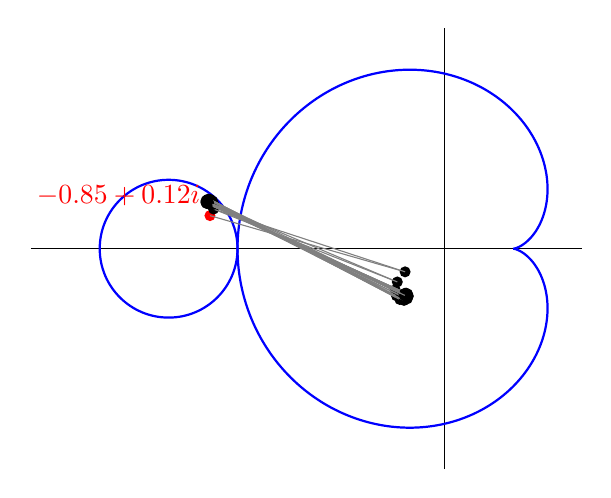
\begin{tikzpicture}[scale=3.5]
% Parámetro c
\def\cre{-0.85}
\def\cim{0.12}

% Ejes (ajustados para ver bien el disco de periodo 2)
\draw(-1.5,0) -- (0.5,0);
\draw (0,-0.8) -- (0,0.8);

% Cardioide principal
\draw[thick,blue,smooth,domain=0:360,samples=400]
plot ({0.5*cos(\x) - 0.25*cos(2*\x)},
      {0.5*sin(\x) - 0.25*sin(2*\x)});

% Disco de 2-ciclo (radio 0.25 centrado en -1)
\draw[thick,blue,smooth] (-1,0) circle[radius=0.25];

\pgfmathsetmacro{\x}{\cre}
\pgfmathsetmacro{\y}{\cim}

% Punto inicial c
\fill[red](\x,\y) circle (0.02) node[above left] {$\x+\y i$};

% Iteraciones 
\foreach \n in {1,...,30} {

    % Calcular z_{n+1}
    \pgfmathsetmacro{\xn}{\x*\x - \y*\y + \cre}
    \pgfmathsetmacro{\yn}{2*\x*\y + \cim}

    % Dibujar segmento
    \draw[gray] (\x,\y) -- (\xn,\yn);

    % Dibujar puntos
    \fill[black] (\xn,\yn) circle (0.02);

    % Actualizar valores
    \xdef\x{\xn}
    \xdef\y{\yn}
}
\end{tikzpicture}
\quad
% ===================== FIGURA 2: c = -1 + 0.10i =====================
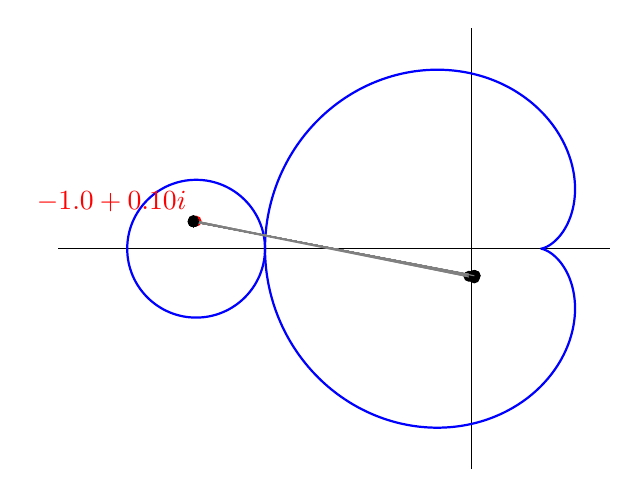
\begin{tikzpicture}[scale=3.5]
% Parámetro c
\def\cre{-1.}
\def\cim{0.10}

% Ejes
\draw(-1.5,0) -- (0.5,0);
\draw (0,-0.8) -- (0,0.8);

% Cardioide principal
\draw[thick,blue,smooth,domain=0:360,samples=400]
plot ({0.5*cos(\x) - 0.25*cos(2*\x)},
      {0.5*sin(\x) - 0.25*sin(2*\x)});

% Disco de 2-ciclo (radio 0.25 centrado en -1)
\draw[thick,blue,smooth] (-1,0) circle[radius=0.25];

\pgfmathsetmacro{\x}{\cre}
\pgfmathsetmacro{\y}{\cim}

% Punto inicial c
\fill[red](\x,\y) circle (0.02) node[above left] {$\x+\y i$};

% Iteraciones 
\foreach \n in {1,...,30} {

    % Calcular z_{n+1}
    \pgfmathsetmacro{\xn}{\x*\x - \y*\y + \cre}
    \pgfmathsetmacro{\yn}{2*\x*\y + \cim}

    % Dibujar segmento
    \draw[gray] (\x,\y) -- (\xn,\yn);

    % Dibujar puntos
    \fill[black] (\xn,\yn) circle (0.02);

    % Actualizar valores
    \xdef\x{\xn}
    \xdef\y{\yn}
}
\end{tikzpicture}
\end{document}